\subsection{Measuring the time to access datas}

We will see two type of histograms that give us informations about the flow of data transfer. But first let us explain how is working the code.\\

First get the url of a .root file you want to read, we will call it "http://url". The idea of the program is to open the file, select a tree \textit{"physics"} and read all the events of the branches \textit{"el\_n"} and \textit{"mu\_n"}. When an event is read we get the time from the beginning of reading and save it. When the branches are fully read, we create an histogram with the times we measured. This histogram has bins of 1 second and their value corresponds to the number of event read during this second.\\

The code is mainly divided in two functions:

\lstset{language=c++}
\begin{lstlisting}[frame=single,framerule=0pt]
	vector<int> fillTimes(char* fileName);
\end{lstlisting}

The takes in argument the url of the file, and return the vector of times. This funcion is the one that opens the file, select the branch we want to read, and finally read them saving the current time.\\


\begin{lstlisting}[frame=single,framerule=0pt]
	void createHistogram(vector<int> datas,char* nameFile, char* nameSite, char* nameProcessor);
\end{lstlisting}

takes in argument:

\begin{itemize}
	\item \textit{datas}: The times we got from \textit{fillTimes}
	\item \textit{nameFile}: The name of the .root file that will be generated
	\item \textit{nameSite}: Name of the site where we are reading (for the title)
	\item \textit{nameProcessor}: Name of the processor where it is running (for the title)
\end{itemize}

This function doesn't return anything because the outputs are generated where the file is. Finally the main function is:

\begin{lstlisting}
	int main(int argc, char* argv[])
	{
		vector<int> timeDatas;
		timeDatas = fillTimes(argv[1]);
		createHistogram(timeDatas,getFileName(argv[1]),getSite(argv[1]), argv[2]);
		return 0;
	}
\end{lstlisting}

where:

\begin{itemize}
	\item \textit{argv[1]} = "http://url"
	\item \textit{argv[2]} = Name of the processor
\end{itemize}

\textit{getFileName(string url)} extract the name of the file from "http://url" and \textit{getSite(string url)} extract the name of the site where we are reading from "http://url".\\

Figure ~\ref{fig:timeHistogram} shows an example of data access in function of the time, the program ran on lxplus and read at DESY\_ZN. In section ~\ref{sec:results} there are more histograms and comments on the results.\\

\begin{figure}
	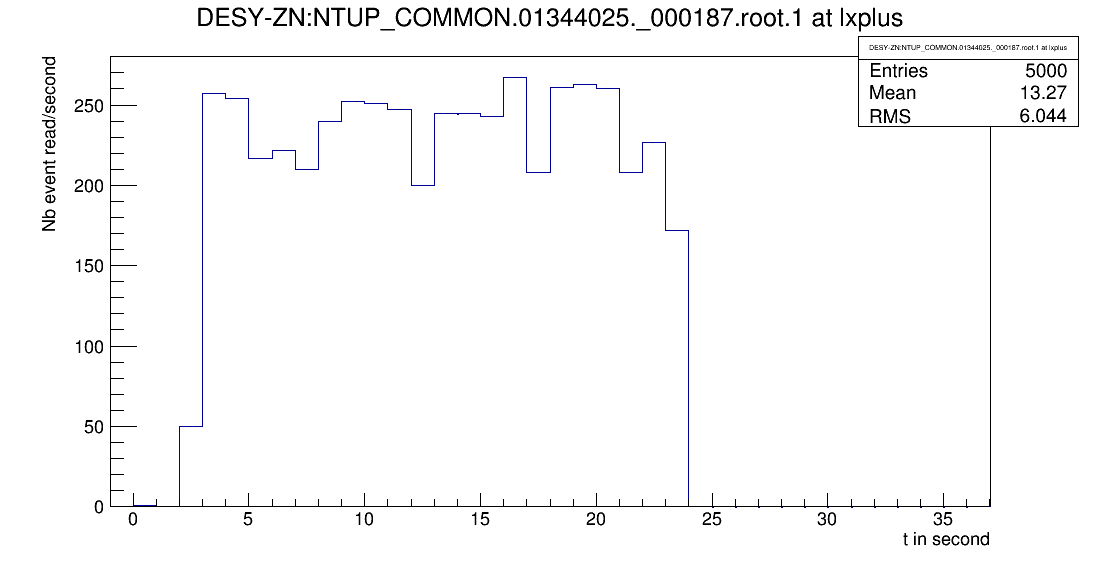
\includegraphics[width=1.1\textwidth]{timeHistogramDESYZN}
	\caption{Flow of Events read for each second at DESY\_ZN}
	\label{fig:timeHistogram}
\end{figure}


We can now see the evolution in the time of remote data access. But we have no idea of if we repeat the experiment the result will be the same, in other words we want to have some stastistics informations about the flow of datas. The idea is simply to repeat this experiment many times. To do that we will stop getting the time to each event reading but we will only get the time to get all datas, which corresponds to the last value of the vector in the previous case.\\

The functions are the same, with little differences:

\begin{itemize}
	\item \textit{fillTimes} will return only one \textit{int} which corresponds to the time to get all datas.\\
	\item \textit{createHistogram} will create an histogram only if none exists with the same processing site (where it runs) and the same read site. If this one already exists the function just open it and append the time divided by we just got. \\
\end{itemize}

This means that our histogram will not give evolution in time but the mean of events read per second, that will be called \textbf{events rate}. While we repeat the experiment the events rate of the file will be added to the histogram. In figure \ref{fig:eventsrateatDESYZNtoLRZ} the program was repeated 100 times, we can see a gaussian with a statistic error and a mean events rate.


\begin{figure}
	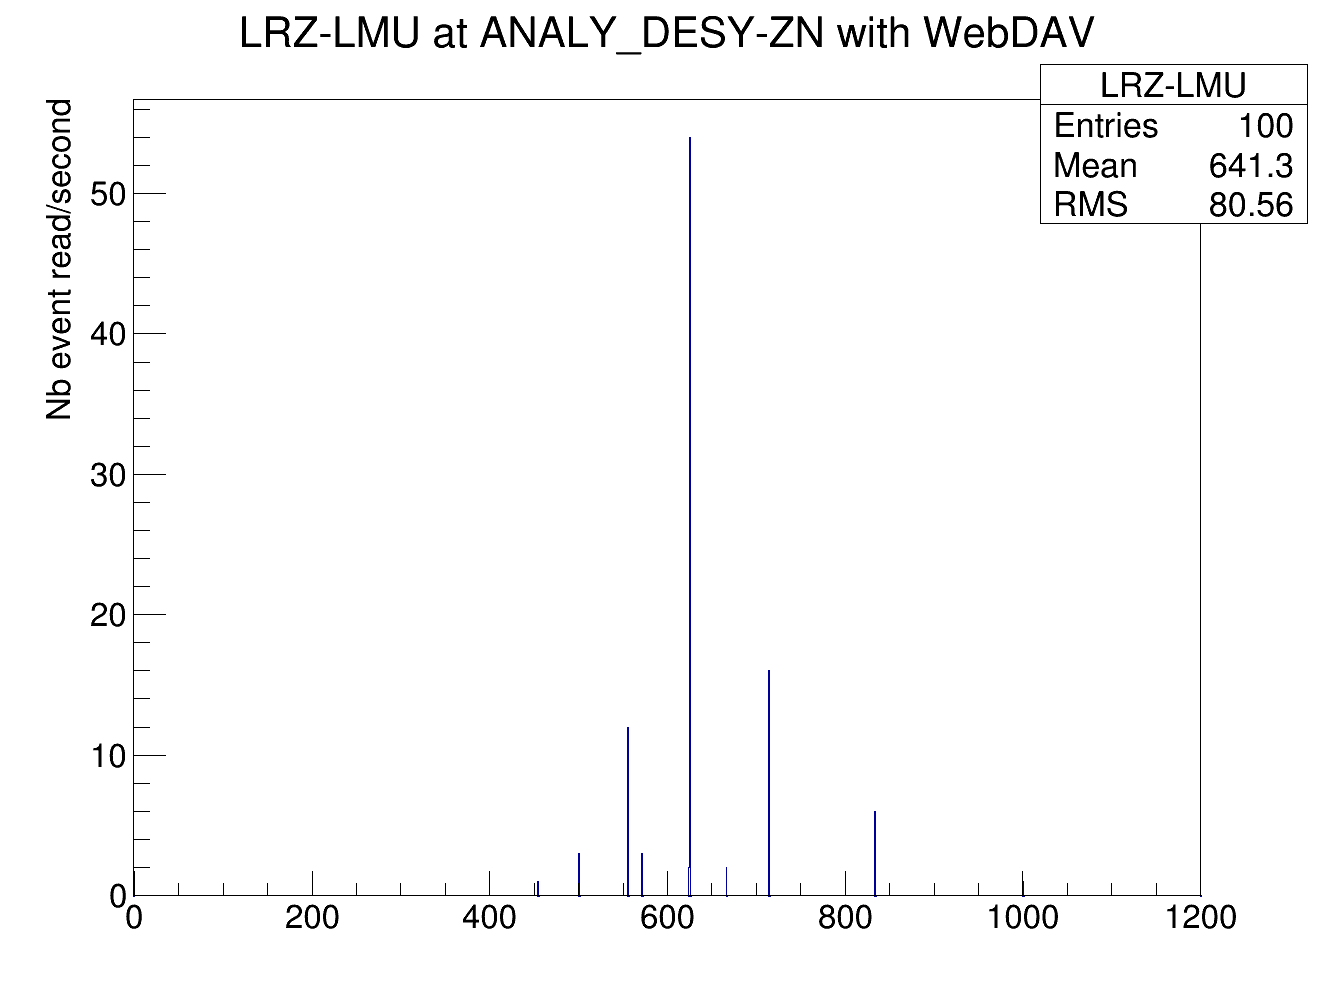
\includegraphics[width=1.1\textwidth]{eventsrateatDESYZNtoLRZ.png}
	\caption{100 events read at LRZ, processed at DESY} 
	\label{fig:eventsrateatDESYZNtoLRZ}
\end{figure}
